\documentclass[tikz, margin=6pt]{standalone}
\usepackage{tikz}
\usepackage{pgfplots}
\usepackage{pgf-spectra}
\usetikzlibrary{arrows}
\usetikzlibrary{angles}
\usetikzlibrary{quotes}
\usetikzlibrary{decorations.markings}

\tikzset{>=latex}

\def \plotwidth {510.0pt}
\def \tth{3.16227766017}

\definecolor{color1}{RGB}{202,0,32}
\definecolor{color2}{RGB}{244,165,130}
\definecolor{color3}{RGB}{146,197,222}
\definecolor{color4}{RGB}{5,113,176}

\newcommand{\styleone}{densely dotted}
\newcommand{\styletwo}{densely dashed}
\newcommand{\stylethree}{dashdotted}
\newcommand{\stylefour}{solid}
\newcommand{\stylefive}{loosely dashed}

\def\linethickness{0.8pt}

\begin{document}
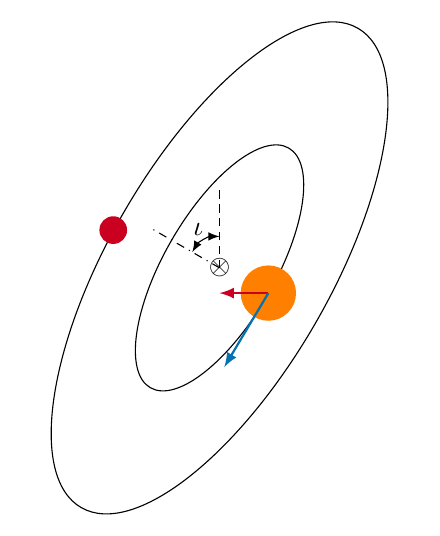
\begin{tikzpicture}[]
    \draw[rotate=60] (0, 0) ellipse (100pt and 40pt);
    \draw[rotate=60] (0, 0) ellipse (50pt and 20pt);
    \node[draw=none] at (0, 0) (a) {$\otimes$};
    \draw[fill=orange, draw=none] (0.62, -0.32) circle (10pt);
    \draw[->, color1, line width=\linethickness] (0.62, -0.32) -- +(-0.62, -0.0);
    \draw[->, color4, line width=\linethickness] (0.62, -0.32) -- +(-0.56, -0.94);
    \draw[fill=color1, draw=none] (-1.35, 0.48) circle (5pt);
    \coordinate (o) at (0.0, 0.0);
    \coordinate (a) at (-1.73/2, 0.5);
    \coordinate (b) at (0, 1.0);
    \draw[\stylethree] (o) -- (a);
    \draw[\styletwo] (o) -- (b);
    \pic [draw, "$\iota$", angle eccentricity=1.0, angle radius=0.4cm, <->, pic text options={shift={(-2pt, 4pt)}}] {angle=b--o--a};
\end{tikzpicture}
\end{document}